\chapter{Load Generating Tool}
As mentioned in chapter \ref{technological background}, existing load generating tools requires comparatively powerful computing unit to host them. In this project, it is not realistic to host such a vigorous load generator because of the cost from extra virtual machine to be installed. Additionally, if client and server are running in the same cluster, unwelcome network overhead can be avoided in some extent. Although self implemented load generator is limited in its capacity, it can be made up through scaling the load generator instance. As \ref{scale-load-generator} shows, enough load can be brought about by parallel running multiple instances.
\begin{figure}[h]
	\centering
	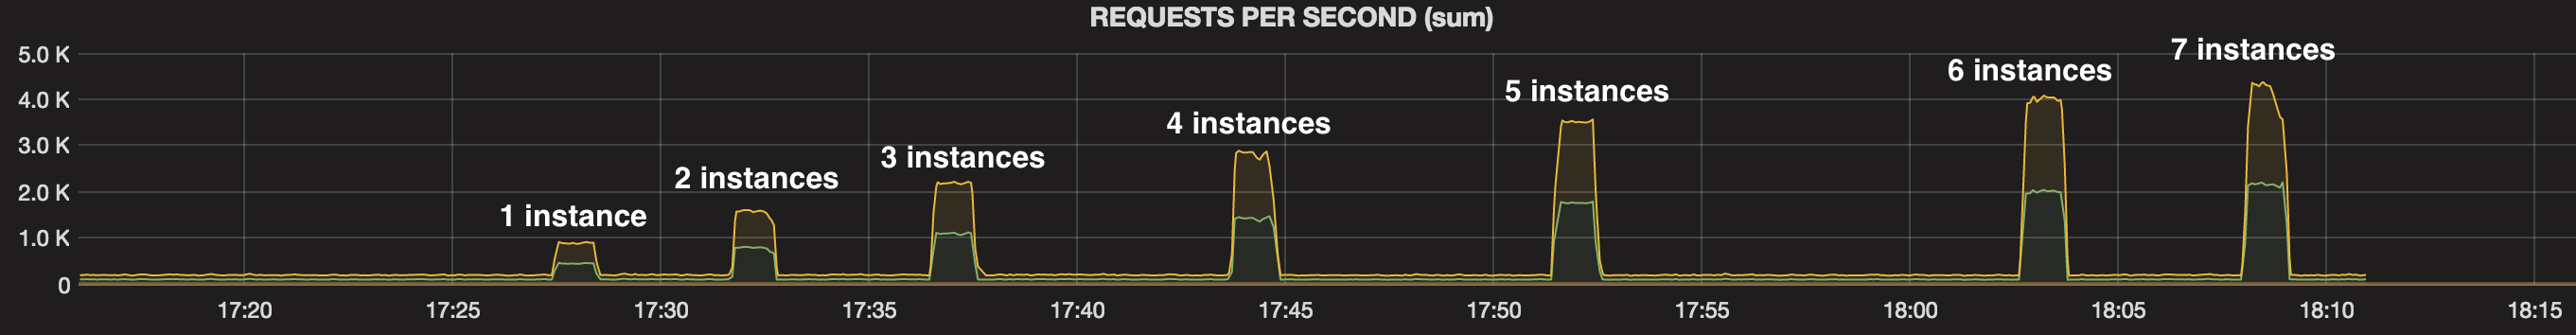
\includegraphics[width=12cm]{scale-load-generator}
	\caption{Load produced from different number of instances}
	\label{scale-load-generator}
\end{figure}

\section{Load generator - a self implemented scalable client}
A simple load generator is implemented in this project as a node application. It sends requests with unique correlation id to the server, records the response time and stores them in database at the end of load generating. Application is deployed to cloud foundry and uses PostgreSQL backing service. A time-out mechanism is added to make sure load is generated in the given time frame. Except for producing fancy graphic analysis results, it pretty much accomplishes every thing a load generating tool can do. It is more flexible to work with raw data anyway.
\missingfigure{Add figure for node application for load generator}
\subsection{Limitations}
Since load generator is deployed as a worker in cloud foundry, it has little choice over database selection. In this project, a docker container version of database is used owing to the fact that other dedicated backing services are not free of charge. There are times container is under great stress and stops running. \\
Secondly, load generator can be resource consuming as already discussed. In Cloud Foundry, some organization or space has only so much memory to provide. It could be hard to scale the load generator to ideal capacity. For example, for a period of time the load testing is conducted in a staging landscape of Cloud Foundry with a limited space quota of 10 G memory. Imagine all the applications and load generators scaling together, the space limit is easily exceeded. \\
Last but not the least, there is a chance the load generator is running on the same node as applications which will directly influence the CPU share the application could obtain resulting in tainted test results. 

